% fig08_tier_dist.tex — Verify-ledger tier distribution bar chart.
% Compiled by the paper Makefile via `make figures` (pdflatex on the snippet).
%
% Data: Appendix G (Verification Ledger), companion/verify-ledger.json.
% The 36-atom ledger partitions by atom_class:
%   20  SUPPORTED-NUMERICAL (green)  -- libm-class recomputes
%    8  SUPPORTED-FORMAL    (blue)   -- BLUE-MAX algebraic-root attestations
%    8  FALSIFIED           (red)    -- matched negative controls (kept as evidence)
% Sum = 36 atoms across 8 landing PRs.
%
% Manual single-shot compile (debug):
%   pdflatex -interaction=nonstopmode -halt-on-error fig08_tier_dist.tex
\documentclass[border=4pt]{standalone}
\usepackage{tikz}
\usepackage{pgfplots}
\pgfplotsset{compat=1.18}
\begin{document}
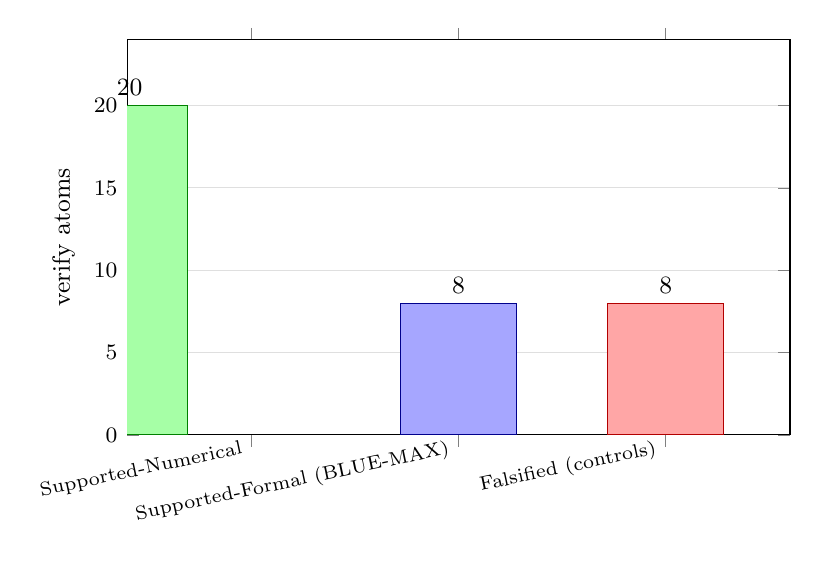
\begin{tikzpicture}
\begin{axis}[
  width=10cm, height=6.6cm,
  ybar,
  bar width=42pt,
  ymin=0, ymax=24,
  ylabel={verify atoms},
  symbolic x coords={Numerical, Formal, Falsified},
  xtick={Numerical, Formal, Falsified},
  xticklabels={Supported-Numerical, Supported-Formal (BLUE-MAX), Falsified (controls)},
  x tick label style={font=\scriptsize,rotate=12,anchor=east},
  tick label style={font=\footnotesize},
  label style={font=\small},
  nodes near coords,
  nodes near coords style={font=\small},
  ymajorgrids,
  grid style={gray!25},
  enlarge x limits=0.30,
]
\addplot[draw=green!50!black,fill=green!35] coordinates {(Numerical,20)};
\addplot[draw=blue!55!black,fill=blue!35,bar shift=0pt] coordinates {(Formal,8)};
\addplot[draw=red!70!black,fill=red!35,bar shift=0pt] coordinates {(Falsified,8)};
\end{axis}
\end{tikzpicture}
\end{document}
